\chapter{Conclusioni}
\lhead{\emph{Capitolo 4}}
In questo capitolo verranno verificate le premesse e gli obiettivi dati all'inizio della tesi. In particolare verrà riportata l'analisi sulle tecnologie web per lo sviluppo ibrido multipiattaforma, mettendo a confronto gli altri metodi di sviluppo analizzati.
Verranno spiegati i cambiamenti che ci sono stati sul processo di sviluppo, avendo prefissato l'obiettivo di avere una applicazione mutlipiattaforma e quali ottimizzazioni sono state adottate. 

\section{Ibrido vs Nativo}
L'obiettivo di questa tesi è stato fin da subito di trovare delle metodologie rapide per sviluppare applicazioni multipiattaforma. L'approccio che è stato analizzato comprendeva l'utilizzo di tecnologie web per applicazioni ibride.
Effettivamente tramite l'impiego degli opportuni framework per la distribuzione di più piattaforme, è stato possibile partendo da un unico codice sorgente in HTML / CSS / Javascript ottenere il risultato desiderato.
Come spiegato nella sezione \ref{sec:native_vs_web} ci sono pro e contro sull'utilizzo di tecnologie web per lo sviluppo di applicazioni mobile. Tramite l'approccio ibrido è stato possibile combinare i vantaggi di questi due approcci, ma fino ad un certo punto. Nella tabella \ref{tbl:html5_vs_native} si possono osservare vantaggi e svantaggi derivati dai due approcci.

\begin{table}[h]
	\centering
	\begin{tabular}{|p{7.5cm}p{7.5cm}|}
		\hline
		\multicolumn{2}{|c|}{\textbf{Applicazioni}} \\ \hline
		\multicolumn{2}{|c|}{\cellcolor{black!10}\textbf{Ibride}}	  \\ \hline
  \cellcolor{green!35}
  \textbf{Pro} 
&
  \cellcolor{red!55}
  \textbf{Contro} 
\\ \hline
  \cellcolor{blue!25} 
  Le tecnologie web hanno una curva di apprendimento più bassa. Gli sviluppatori che vogliono usare tecnologie web per creare applicazioni mobile, impiegano meno tempo ad imparare il linguaggi (HTML / CSS / JS) rispetto ad uno nativo.
&
  \cellcolor{blue!10}
  Essendo Javascript un linguaggio interpretato all'interno della WebView di Webkit, sarà comunque meno performante di un linguaggio nativo compilato, pur essendo Webkit una WebEngine molto efficiente. 
\\
  \cellcolor{blue!10}
  Permette di avere da un unico sorgente, un'applicazione per ciascuna piattaforma, senza dover riscrivere il codice.
&
  \cellcolor{blue!25}
  Pur essendo un linguaggio facile, non si hanno strumenti altrettanto potenti 
  per poter fare debug del codice e memory profiling (anche se ultimamente stanno nascendo tool molto interessanti).
\\
  \cellcolor{blue!25}
  Grazie ai punti precedenti, può permettere un risparmio di tempi e costi, specialmente per la creazione di applicazioni multipiattaforma.
&
  \cellcolor{blue!10}
  L'accesso alle funzionalità native del dispositivo è vincolato dal wrapper che fornisce le API in Javascript. Dipende quindi dalla tecnologia che si va ad utilizzAppendiceare.
\\\hline		
        \multicolumn{2}{|c|}{\cellcolor{black!10}\textbf{Native}} \\ \hline
  \cellcolor{green!35}
  \textbf{Pro} 
& 
  \cellcolor{red!55}
  \textbf{Contro} 
\\ \hline
  \cellcolor{blue!10}
  Tramite il linguaggio nativo della piattaforma, si può ottenere la massima performance in termini di potenza di calcolo e di sfruttamento del processore. 
& 
  \cellcolor{blue!25}
  E’ necessario riscrivere l'applicazione per ogni piattaforma che si intende supportare.
\\
  \cellcolor{blue!25}
  Sfrutta tutte le caratteristiche specifiche della piattaforma, sia in termini di software (librerie del produttore o di terze parti) che di hardware (del dispositivo o esterno)
&
  \cellcolor{blue!10}
  Richiede conoscenze specifiche dei vari linguaggi delle varie piattaforme da parte degli sviluppatori.
\\
  \cellcolor{blue!10}
  Si ha un accesso più a basso livello della piattaforma, cosa che spesso non è consentita alle API per ragioni di sicurezza.
&
  \cellcolor{blue!25}
  A causa dei punti precedenti può comportare un maggiore costo complessivo e l'allungamento dei tempi di sviluppo, in particolare dovendo gestire più piattaforme.
\\ \hline
 
	\end{tabular}
	\caption{HTML5 vs Nativo, pro e contro dei due approcci}
	\label{tbl:html5_vs_native}
\end{table}

Per quanto riguarda la creazione di una interfaccia utente e l'impostazione della user experience, si accusa spesso l'approccio ibrido di non poter garantire un risultato soddisfacente paragonandolo allo sviluppo ibrido. In questo caso mi permetto di dissentire personalmente da questa opinione, in quanto dalla mia esperienza di utilizzo dei framework web per la creazione della UI (come ad esempio IONIC o Foundation), l'interfaccia risulta fluida e accattivante anche se eseguita all'interno di una WebView. Le principali accuse che vengono fatte ad una interfaccia web sono di essre eseguita a scatti, di non garantire una UX ottimale. Se si fa utilizzo di animazioni CSS3 (il quale processo di rendering è accelerato dall'hardware), invece della manipolazione del DOM tramite javascript, la differenza con una applicazione nativa è pressoché nulla.

\section{I cambiamenti sul processo di sviluppo}
I cambiamenti sul processo di sviluppo\\

 - Il progetto è soltanto uno\\
 * Test funzionali unici, da testare solo l'integrazione con i sistemi\\
 * Meno persone dedite al progetto, quindi processo più facile da gestire\\
 * Tutte le applicazioni sono pronte nello stesso momento\\
\section{Ulteriori otimizzazioni dell'approcio ibrido}
Nello sviluppo di una applicazione in generale, tutte le figure professionali coinvolte fanno riferimento ad uno schema generale, che illustra le fasi di lavoro per arrivare al prodotto finale. Da quanto appreso durante l'esperienza di tirocinio in azienda, questo schema deve essere il più generico possibile, e comprensibile da chiunque lavori con esso. Nella figura \ref{fig:classic_app_flow} si possono osservare le fasi principali dello sviluppo di una applicazione.

\begin{figure}
	\begin{center}
		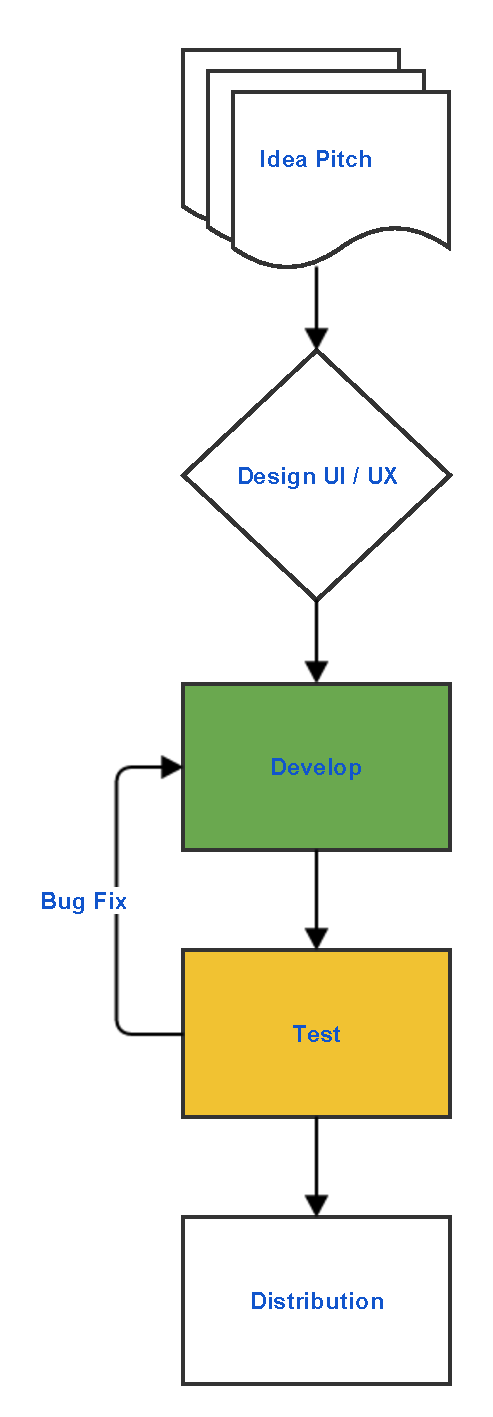
\includegraphics[scale=0.5]{Figures/classic_app_flow.pdf}
		\caption[Schema generale]{In questo schema sono illustrate le fasi generiche dello sviluppo di una applicazione}
		\label{fig:classic_app_flow}
	\end{center}
\end{figure}

Prendendo spunto da questo schema generale ho creato una espansione della fase di sviluppo e di test per lo sviluppo di applicazioni multipiattaforma ibride. Si tratta di un sottoschema che evidenzia quali fasi hanno caratterizzato un primo approccio a questo tipo di sviluppo.
Una prima fase è stata quella di scegliere quali tecnologie web utilizzare per lo sviluppo ibrido, e quali per per testare il codice che doveva essere prodotto. Nel mio caso il framework AnagularJS si prestava già ad uno sviluppo di questo tipo e non ho impiegato molto tempo nel capire come utilizzarlo per lo sviluppo mobile. In altri casi, data la vasta scelta di framework javascript per lo sviluppo mobile, la scelta può richiedere parecchio tempo(dipende dalle competenze e dallo stile del programmatore).
Dopo aver costruito il mio ambiente di sviluppo ho proceduto come nello schema \ref{fig:classic_app_flow} sviluppando e testando l'applicazione.

Certamente iterare questo processo per ciascuna applicazione che si andrà a sviluppare è molto dispendioso in termini di tempo e risorse. Una buona soluzione e costruirsi un set di tecnologie che si andranno a utilizzare per lo sviluppo di ciascuna applicazione futura, quello che in azienda si è chiamato \emph{skeleton}. Ovviamente lo scheletro di una applicazione tipo deve essere fatto in modo da espandersi nel caso giungessero richieste di nuove caratteristiche non ancora incluse. Nella figura \ref{fig:flow_match} si può osservare l'evoluzione del primo schema verso una soluzione pronta e rapida all'utilizzo, grazie all'introduzione dello \emph{skeleton}.
HTML5 vs Nativo

\begin{figure}
	\begin{center}
		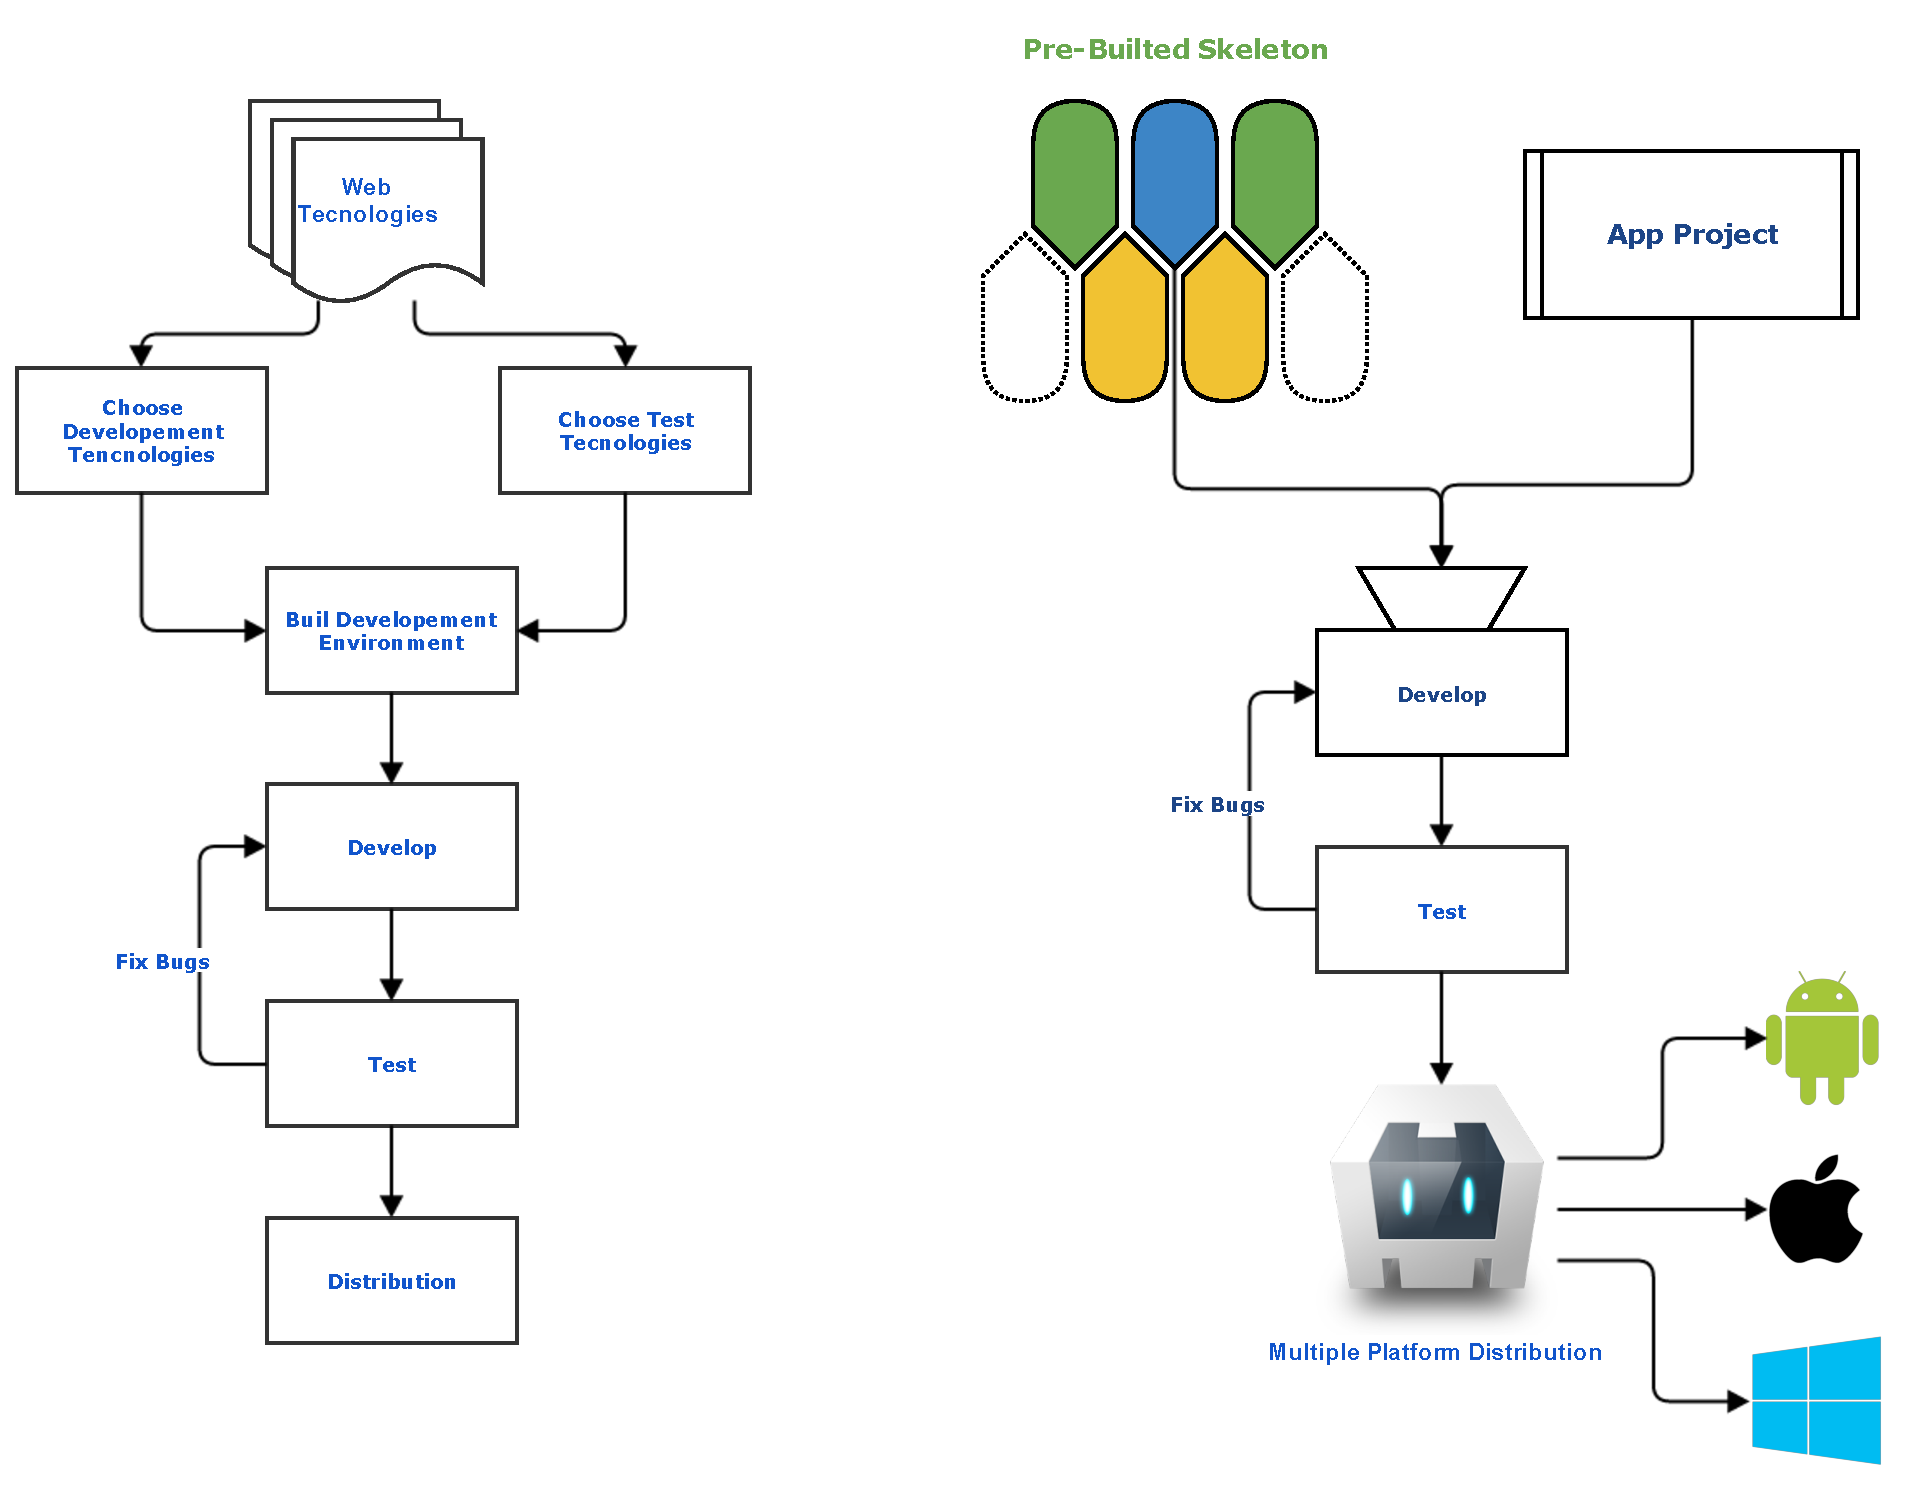
\includegraphics[scale=0.5]{Figures/match_flow.pdf}
		\caption[Schemi di sviluppo a confronto]{Questo schema illustra l'evoluzione del primo schema verso una struttura più completa e multipiattaforma}
		\label{fig:flow_match}
	\end{center}
\end{figure}

Adottare questa pre-configurazione di tutte le tecnologie, mi ha portato a definire delle caratteristiche che lo scheletro di una applicazione deve avere, indipendentemente dalle tecnologie e i linguaggi utilizzati:

\begin{description}
\item[Dipendenze] Lo scheletro di una applicazione deve specificare tutte le dipendenze con software o pacchetti esterni.

\item[Modulare] Se un certo numero di applicazioni richiedono una nuova funzionalità che non è ancora inclusa nello scheletro, ci deve essere la possibilità di poterla aggiungere per tutte le applicazioni future. Al contrario non tutti i nuovi moduli devono per forza essere inclusi nelle implementazioni successive.

\item[Strutturato] Deve avere innanzitutto una struttura ben accurata a livello di directory, in modo tale che i file possano essere separati nella maniera che lo sviluppatore ritiene più opportuna. Ad esempio in AngularJS e possibile separare il codice in diversi moduli. Ci sono diverse linee di pensiero che sostengono che la separazione del codice debba avvenire in maniera semantica per il ruolo che quel modulo ricopre (ad esempio un modulo potrebbe essere la gestione dell'autenticazione con le varie direttive e controller). Altri sostengono che i moduli debbano essere divisi in base al tipo delle struttura utilizzata (sempre nel caso di AngularJS nei vari moduli vengono raggruppati per controller, direttive, service \ldots).
Un metodo molto utilizzato per poi ri-assemblare tutte le parti del codice è tramite l'utilizzo di un task-runner (\ref{sec:task_runner}).

\item[Documentato] Documentare come funziona il proprio scheletro di applicazione e tutte le sue caratteristiche, da modo ai collaboratori futuri di apprendere nel minor tempo possibile il suo funzionamento. Esistono delle tecnologie che, date le giuste annotazioni nel codice, creano già una documentazione chiara e dettagliata.
\end{description} 

\section{Nuove tecnologie web emergenti}

\subsection{FirefoxOS}

\subsection{WebOS}

\subsection{Node Webkit}

\subsection{WebRTC}